\section{Use Case}

This section compares an implementation of a simplified Pac-Man game in Haskell with \dsl{} and TypeScript with GSAP both quantitatively and qualitatively. The quantitative evaluation consists of a comparison of development time and lines of code (LOC). The qualitative compares different aspects of the animation libraries. A screenshot of the application can be seen in Figure~\ref{fig:pacman}.

\begin{figure}[h]{\textwidth}
\centering
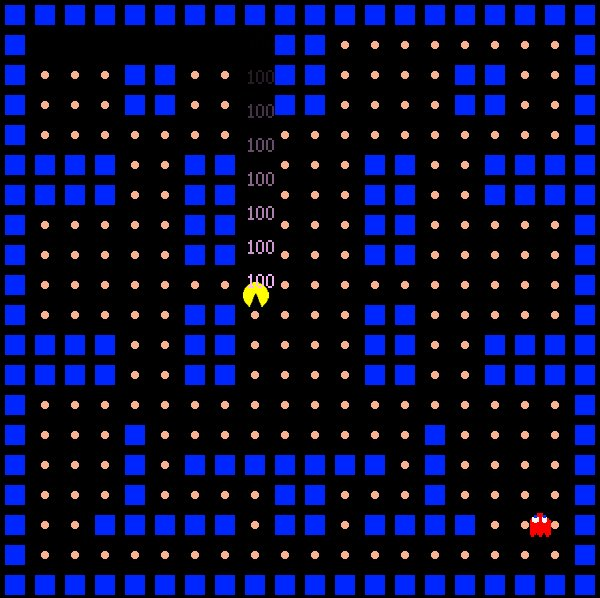
\includegraphics[width=.3\textwidth]{pictures/pacman}
\caption{Screenshot of the Pac-Man application.}
\label{fig:pacman}
\end{figure}

\subsection{Quantitative Evaluation}

This section compares the PaSe and GSAP implementations with respect to certain quantitative criteria. We consider the development time and lines of code for each module.

\begin{itemize}
\item \textbf{Development Time} We roughly kept track of the development time. The development of the Haskell application took $\sim$1.5 working days, while the TypeScript application took $\sim$1 working day. We consider this as the same development time as the Haskell application was developed first, and thus it also contains work shared by both applications.
\item \textbf{Lines of Code} Table~\ref{tbl:loc} contains the lines of code data (including whitespace) for each of the applications. The total lines of code for each of the application is roughly the same. However, the Haskell implementation had to implement some extra code concerning sprites and textures, which was unneeded for the TypeScript application as we utilized the \texttt{Sprite} class of the \texttt{PixiJS} library.
\item \textbf{Relative LOC} Table~\ref{tbl:loc} also contains the relative lines of code. The animation definitions module (AnimDefs) is slightly higher for the GSAP code. We had to embed effects in the animations due to differences in the used graphics library, and the extra verbosity of TypeScript had extra impact in this module. Using the timeline feature of GSAP, the experience for simple animations is comparable to PaSe. However for more complex animations and animations requiring embedded effects, there are some differences. We discuss this in more detail in the qualitative evaluation.
\end{itemize}

\begin{table}[t!]
\caption{Lines of code comparison (including whitespace)}
\centering
\label{tbl:loc}
\begin{center}
\begin{tabular}{l@{\hskip 0.5cm}ll@{\hskip 0.2cm}ll}
 Module & Haskell/PaSe (LOC) & \% & TypeScript/GSAP (LOC) & \% \\
 \hline
 AnimDefs & 127 & 21\% & 197 & 32\% \\ 
 Anims & 43 & 7\% & 39 & 6\% \\  
 Field & 48 & 8\% & 77 & 12\% \\  
 Game & 130 & 21\% & 113 & 18\% \\  
 Main & 36 & 6\% & 23 & 4\% \\  
 Sprite & 45 & 7\% & / & / \\  
 Textures & 34 & 6\% & 13 & 2\% \\  
 Types & 10 & 2\% & 3 & 0\% \\  
 View & 139 & 23\% & 158 & 25\% \\
 \emph{Total} & \emph{612} & \emph{100\%} & \emph{623} & \emph{100\%}
\end{tabular}
\end{center}
\end{table}

\subsection{Qualitative Evaluation}

This section compares the PaSe and GSAP with respect to certain qualitative criteria. The criteria we consider are:

\begin{itemize}
\item \textbf{Eco-system} Animations are not created in isolation, there needs to be coupling to a graphical backend to display them on the screen. The GSAP library is well integrated with the browser. It supports a rich set of features such as a variety of plugins, compatibility across browsers and support for tweening a large range of properties. It is clear that the maturity of GSAP makes it a clear winner in this regard. For the Pac-Man use case, the use of lenses sufficed to target properties of our self-defined state data type.
\item \textbf{Workflow} When creating animations it is important that they can be specified easily and in a concise manner. Creating pure animations, without any embedded effects, are equally convenient in GSAP as in PaSe. However, more complex interactions with effects and control flow are simpler in PaSe. We encountered this in the Pac-Man use case when implementing particle animations. A particle animation is an animation which creates an object, applies an animation on it, and after that animation that object is destroyed. We implemented a general wrapper for such animations which takes as input a function \hs{Int -> Animation}, where the \hs{Int} is the unique particle identifier, and a creation and deletion function for the particle. In the GSAP library we have to add the function to the timeline as a callback, which results in the duration being considered as \hs{0}. However, the deletion of the particle should occur after the particle animation. This means that we are forced to manually calculate and provide the duration for the particle animation.
\item \textbf{Performance} In the Pac-Man use case, both libraries function equally acceptable for a game application: no visible glitches or lag at 60 frames per second (FPS). We have also implemented a benchmark similar to GSAP's speed test\footnote{\url{https://greensock.com/js/speed.html}}. This test benchmarks animations with a large amount of parallel components. GSAP is slightly more optimized as it handles 500 parallel animations at 60 FPS, while PaSe currently handles 400 parallel animations at 60 FPS. The tests were done on an Intel core i7-6600U at 2.60 GHz with 8B memory. There are still some approaches for improving performance such as fusing multiple parallel animations or improving the \hs{Animation} data structure that we have not applied yet.
\item \textbf{Extensibility \& Inspectability} One of the main focus points of this paper is the extensibility and inspectability features of PaSe. Here we answer the question whether these concerns were relevant for this use case. The inspectability aspect was useful for extracting all used textures in the animations. By doing this we were able to automate the loading of the needed textures for the application. The particle effect mentioned earlier was created by using the extensibility feature, we created a new \hs{WithParticle} type class and implemented both an \hs{Animation} instance and a \hs{Const} instance for the texture inspection. GSAP has no counterpart to the inspectability feature, and thus we did not implement the automatic tracking of textures. The particle animation function was possible by using implicit arbitrary effects and callbacks.
\end{itemize}
